\documentclass{article}
\usepackage{graphicx}
\usepackage{float}
\usepackage{titlesec}
\usepackage{datetime}
\usepackage{geometry}
\usepackage{placeins}
\usepackage{minted}
\usepackage{xcolor}
\usepackage{listings}
\usepackage{caption}
\usepackage[document]{ragged2e}
\usepackage[hidelinks]{hyperref}
\usepackage{enumitem}
\geometry{
 a4paper,
 left=25mm,
 top=25mm,
 }
\captionsetup{hypcap=false} 
\newdateformat{daymonthyear}{\THEDAY .\THEMONTH .\THEYEAR}
\title{
  \centering
  
\includegraphics[width=\textwidth]{images/logo_PWr_kolor_poziom.png}\\
  \fontsize{28pt}{30pt}\selectfont Sprawozdanie 6\\
  \fontsize{14pt}{30pt}\selectfont Ćwiczenie 6.Układ słoneczny}
\author{Krzysztof Zalewa}
\date{\daymonthyear\today}
\renewcommand*\contentsname{Spis treści}
\renewcommand{\figurename}{Rysunek}
\renewcommand{\listingscaption}{Fragment kodu}
\begin{document}
    \maketitle
    \pagebreak
    \tableofcontents
    \FloatBarrier
    \section{Wstęp teoretyczny}
        \subsection{Układ słoneczny}
            Wielkości planet zostały dobrane eksperymnetacyjnie "tak żeby wyglądały dobrze". Wyjątkiem
            są wartości pochylenia osiowego planet (dokładność do 1 miejsca po przecinku).
            \begin{table}[ht]
                \centering
                \begin{tabular}{|c|c|c|}
                    \hline
                    Planeta & Moja wartość & Wartość rzeczywista \\ \hline
                    Merkury & 0.03      & ~0.034      \\ \hline
                    Wenus   & 177.4*    & ~177.36    \\ \hline
                    Ziemia  & 23.5      & ~23.44     \\ \hline 
                    Mars    & 25.2      & ~25.19     \\ \hline
                    Jowisz  & 3.1       & ~3.13      \\ \hline
                    Saturn  & 26.7      & ~26.73     \\ \hline
                    Uran    & 97.8      & ~97.77     \\ \hline
                    Neptun  & 28.3      & ~28.32     \\ \hline
                    Pluton  & 122.5*    & ~122.53    \\ \hline
                \end{tabular}
                \caption{Pochylenie osiowe planet}
                \label{tab:axial_tilt}
            \end{table}
            \* Wysoki stopień nachylenia sprawia że Wenus i Pluton obracają się 
            zgodnie z ruchem wskazuwek zegara. Pozostałe planety obracają się
            w przeciwną stronę.
        \subsection{Wykorzystane tekstury}
        \begin{figure}[ht]
            \centering
            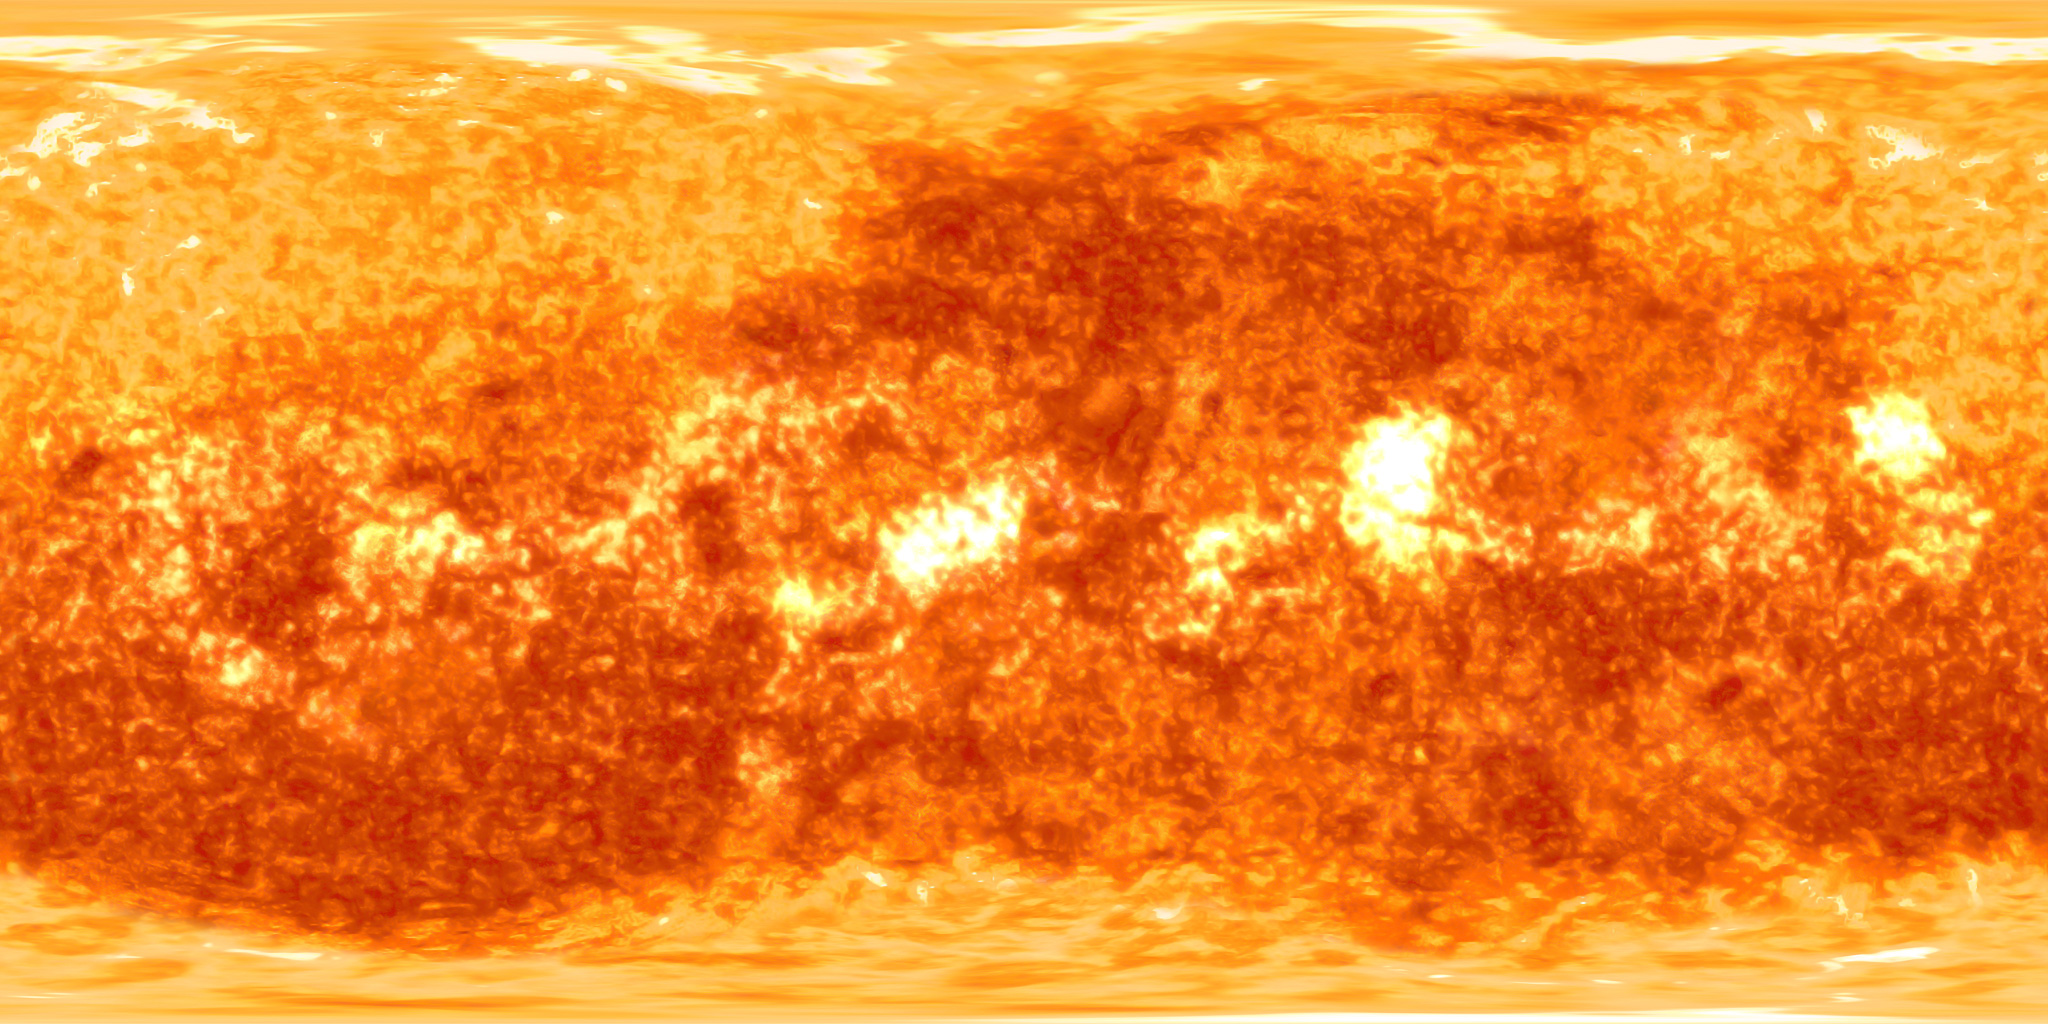
\includegraphics[width=\textwidth]{images/2k_sun.jpg}
            \caption{Tekstura słońca[1]}
            \label{fig:sun}
        \end{figure}
        \FloatBarrier
        \begin{figure}[ht]
            \centering
            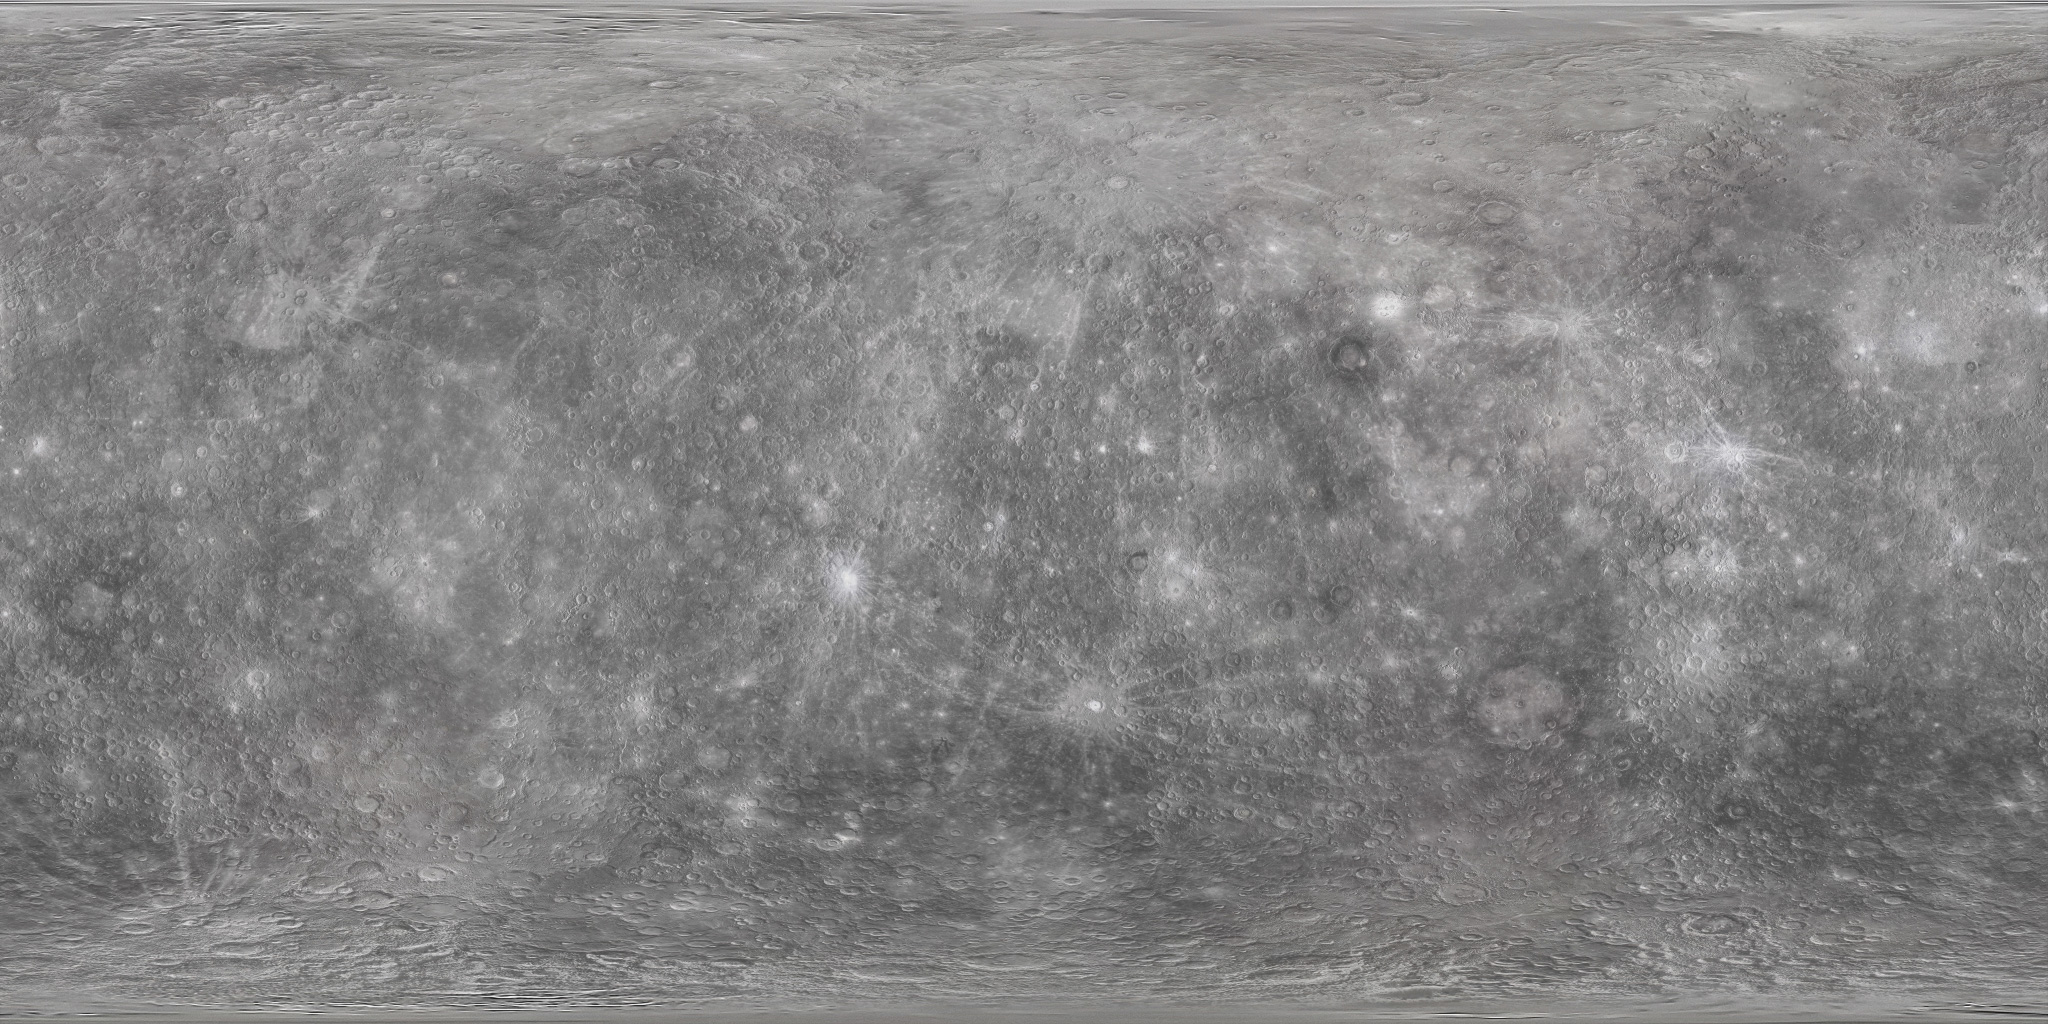
\includegraphics[width=\textwidth]{images/2k_mercury.jpg}
            \caption{Tekstura merkurego[1]}
            \label{fig:mercury}
        \end{figure}
        \FloatBarrier
        \begin{figure}[ht]
            \centering
            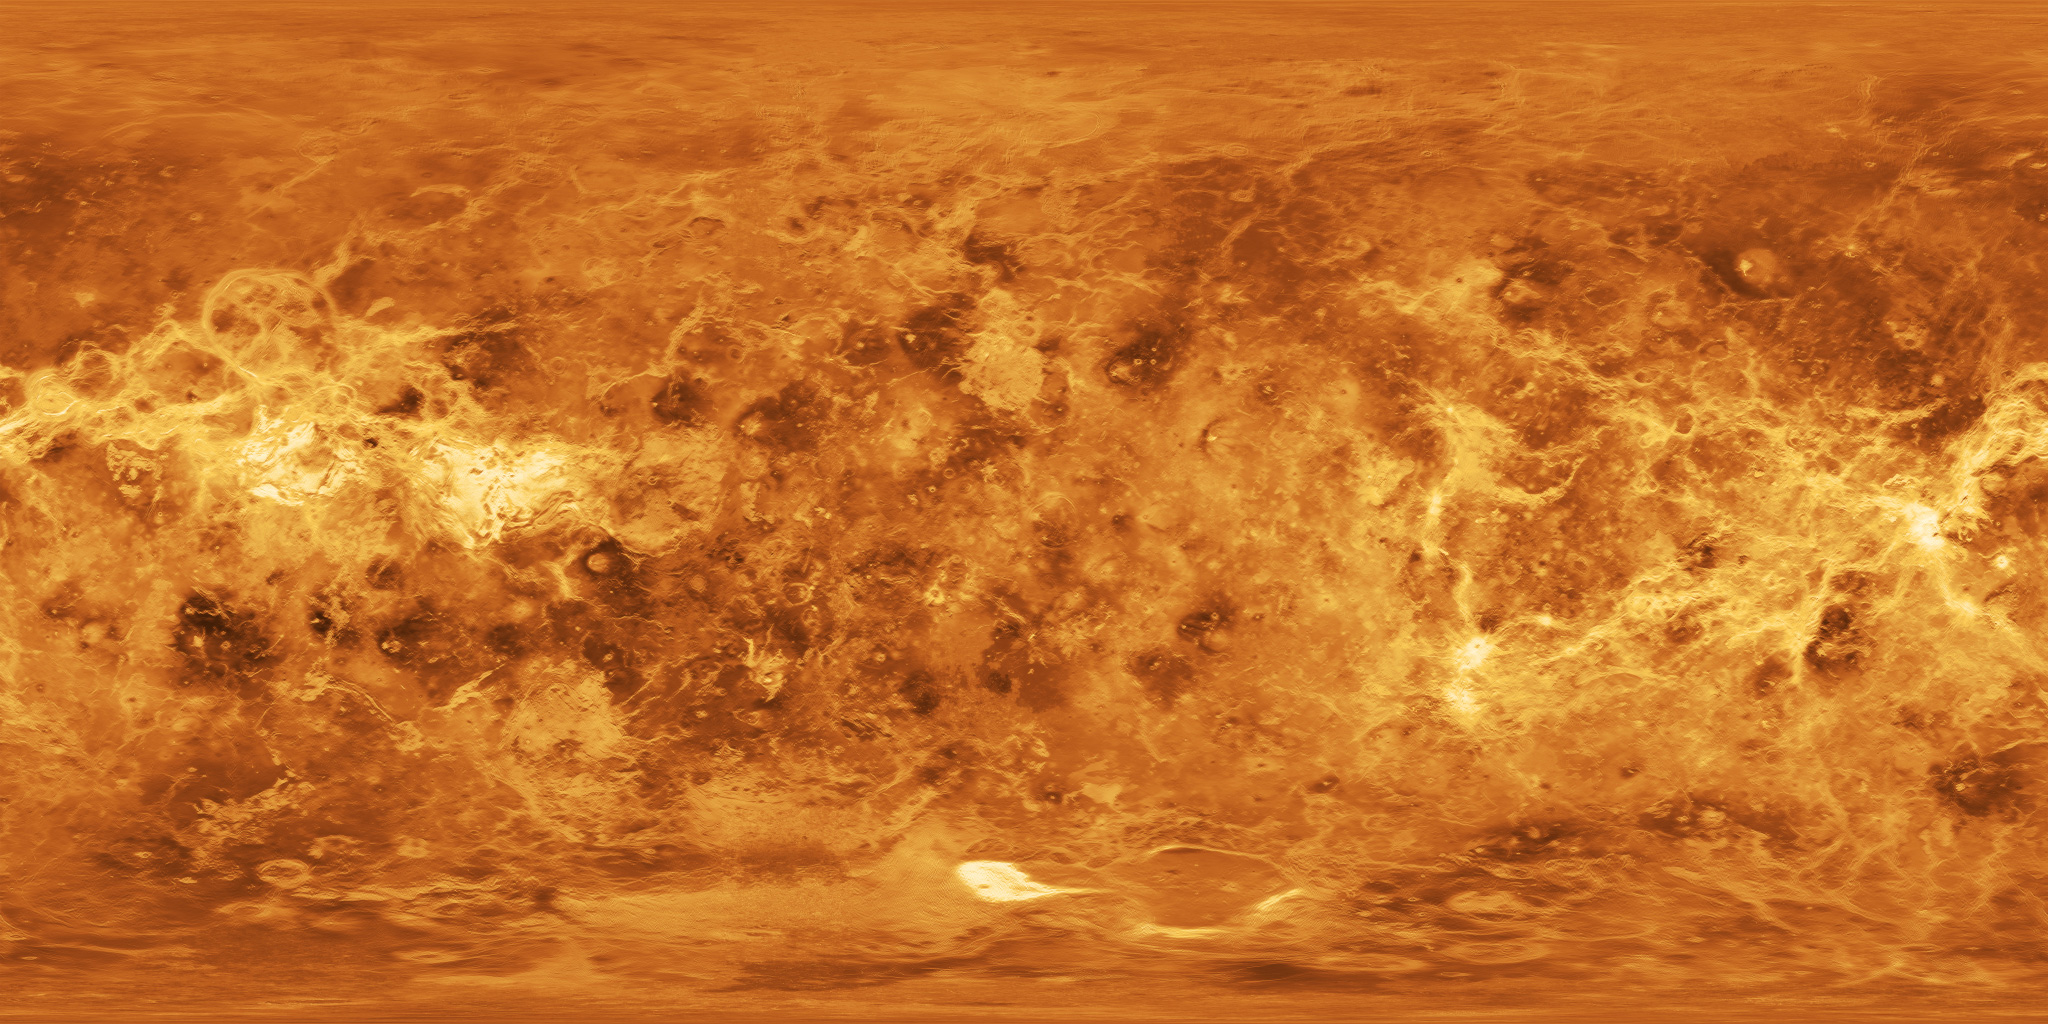
\includegraphics[width=\textwidth]{images/2k_venus_surface.jpg}
            \caption{Tekstura wenus[1]}
            \label{fig:venus}
        \end{figure}
        \FloatBarrier
        \begin{figure}[ht]
            \centering
            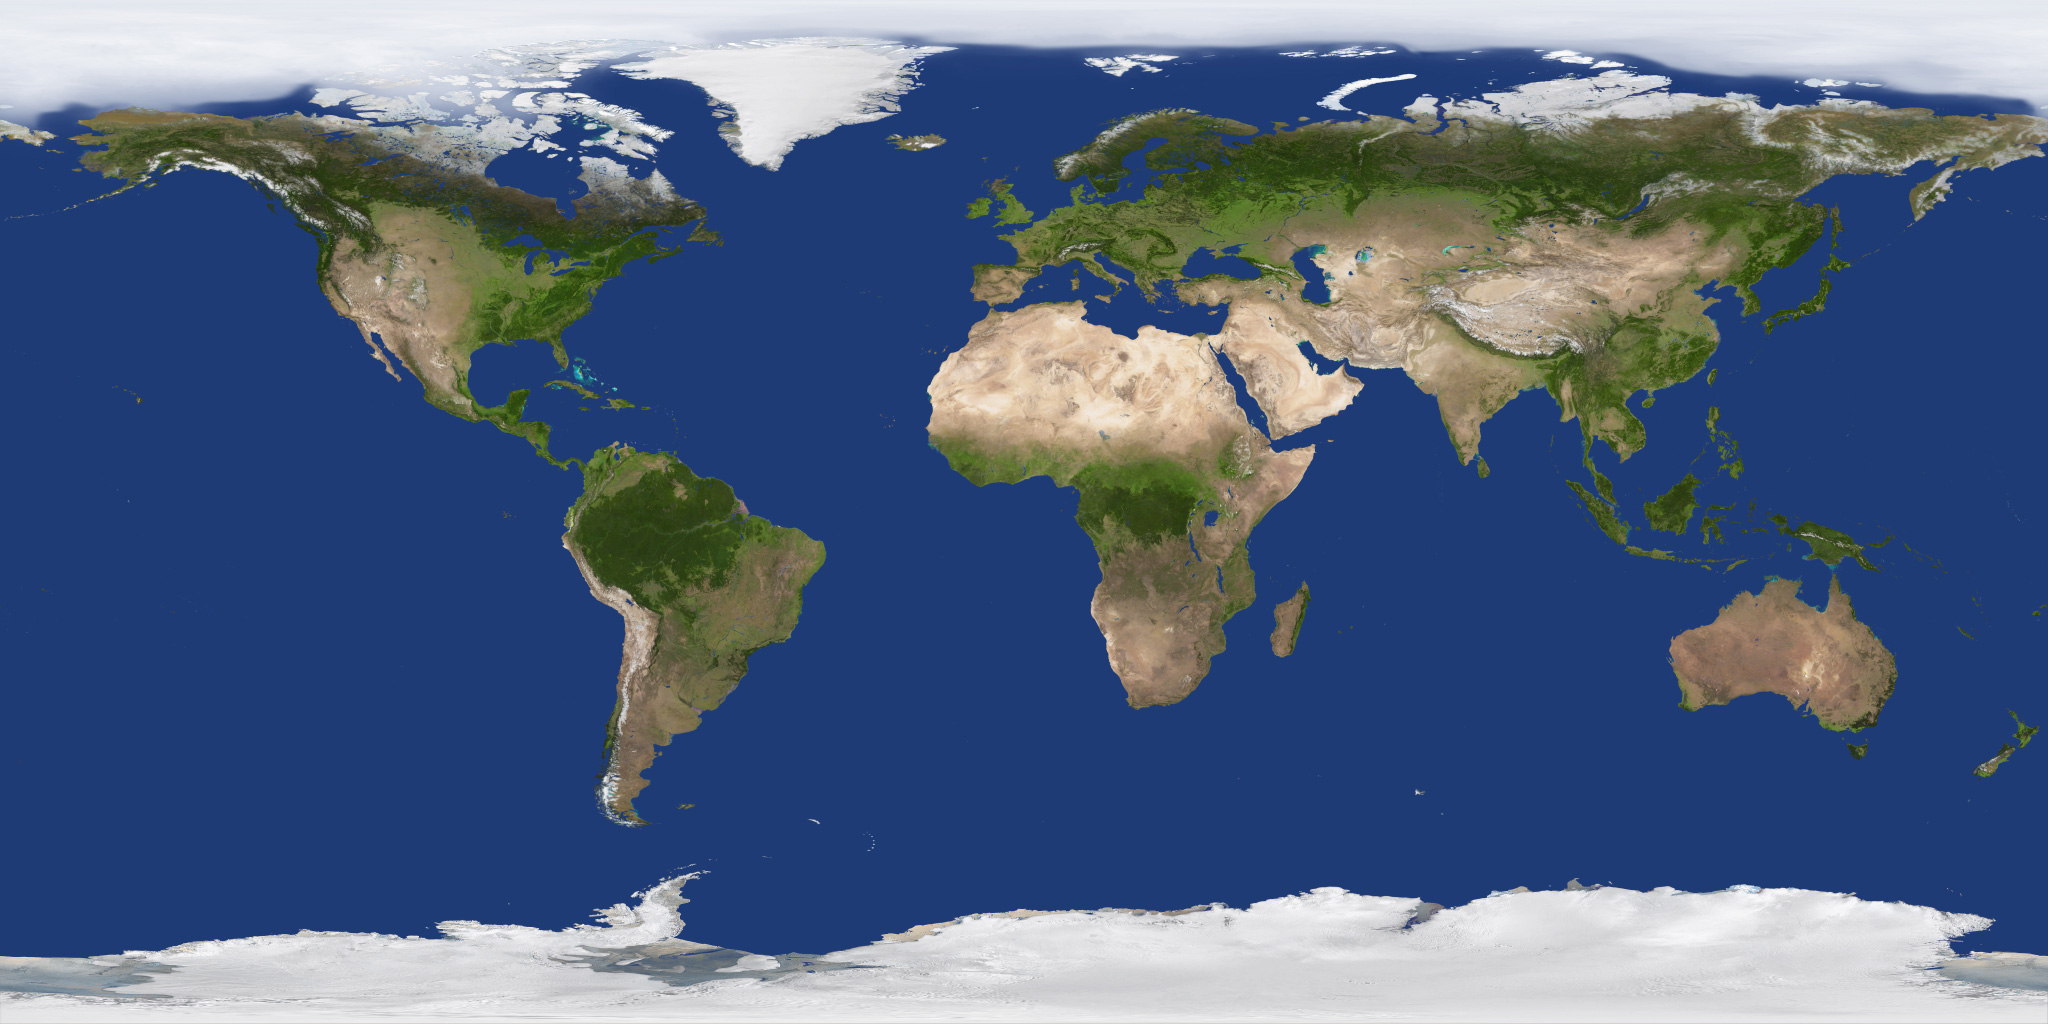
\includegraphics[width=\textwidth]{images/2k_earth_daymap.jpg}
            \caption{Tekstura ziemi[1]}
            \label{fig:earth}
        \end{figure}
        \FloatBarrier
        \begin{figure}[ht]
            \centering
            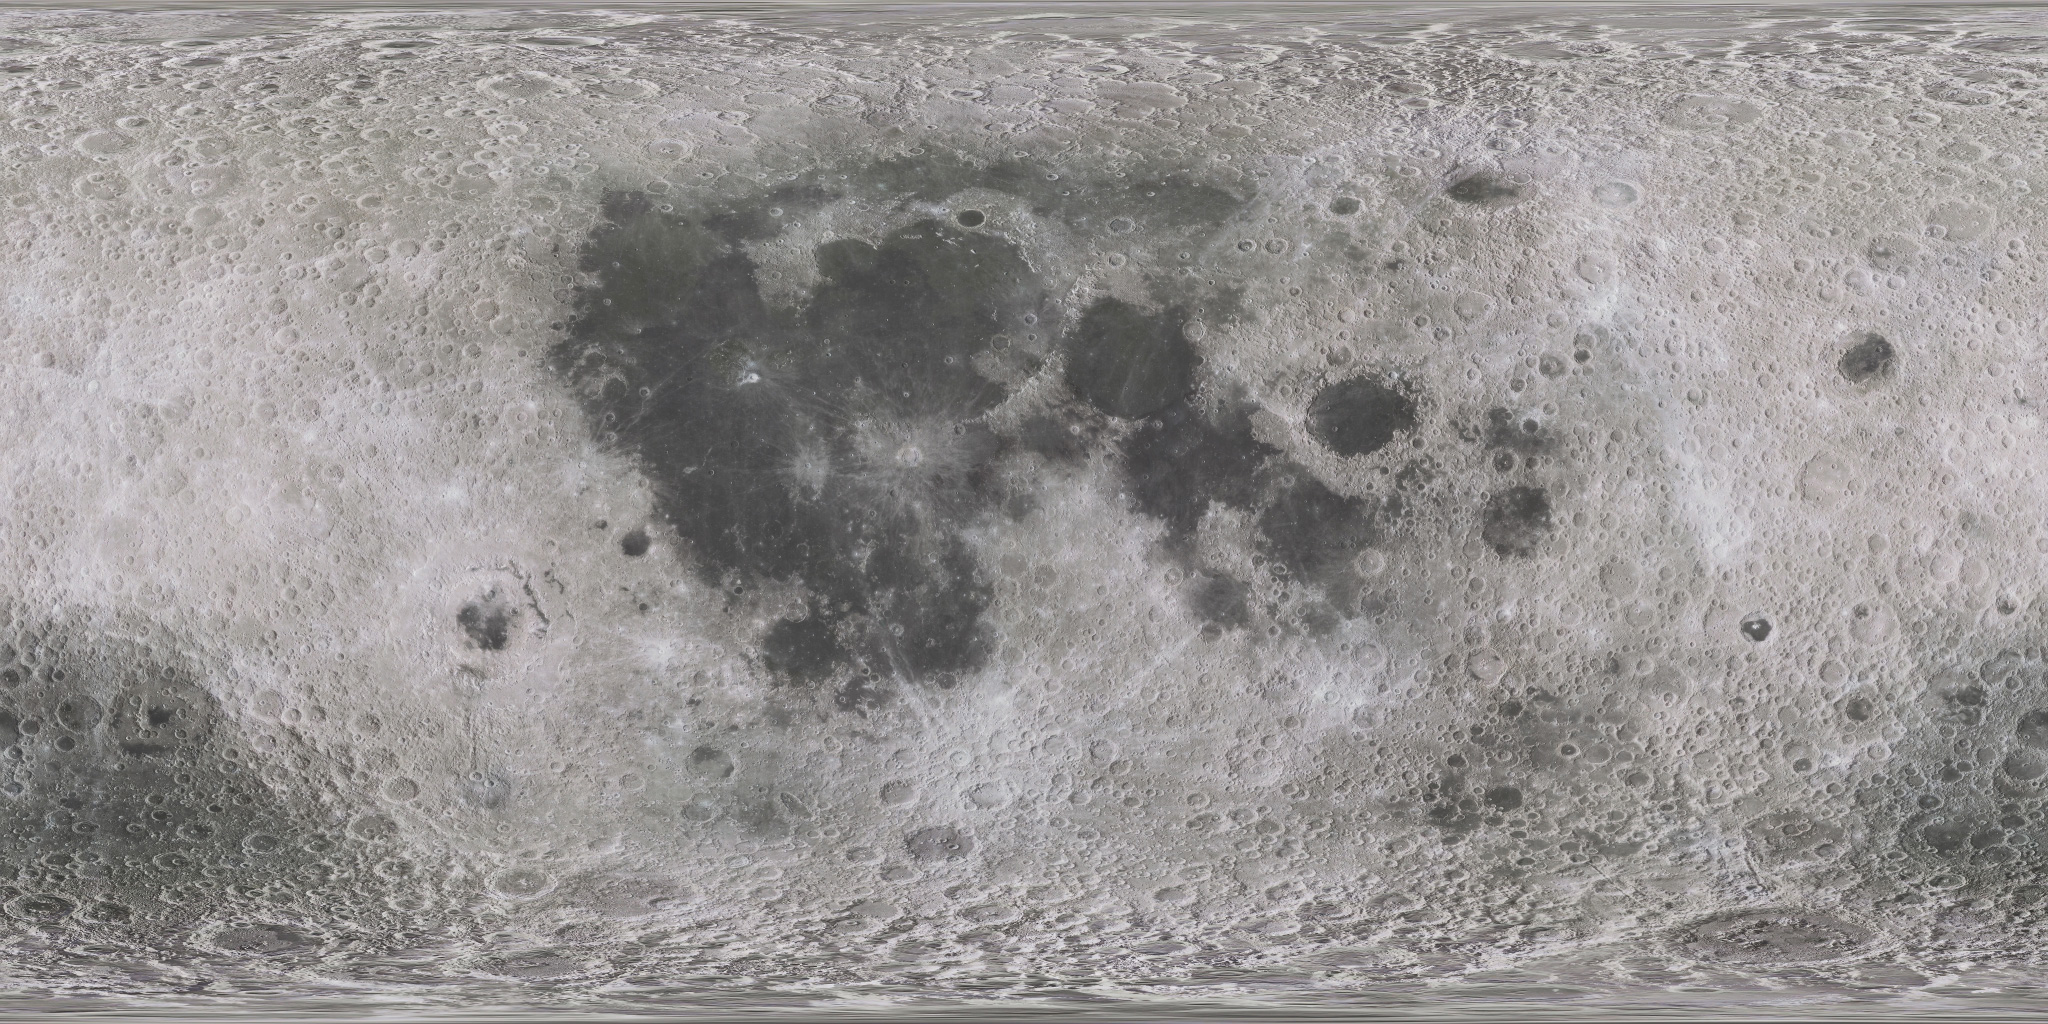
\includegraphics[width=\textwidth]{images/2k_moon.jpg}
            \caption{Tekstura księżyca[1]}
            \label{fig:moon}
        \end{figure}
        \FloatBarrier
        \begin{figure}[ht]
            \centering
            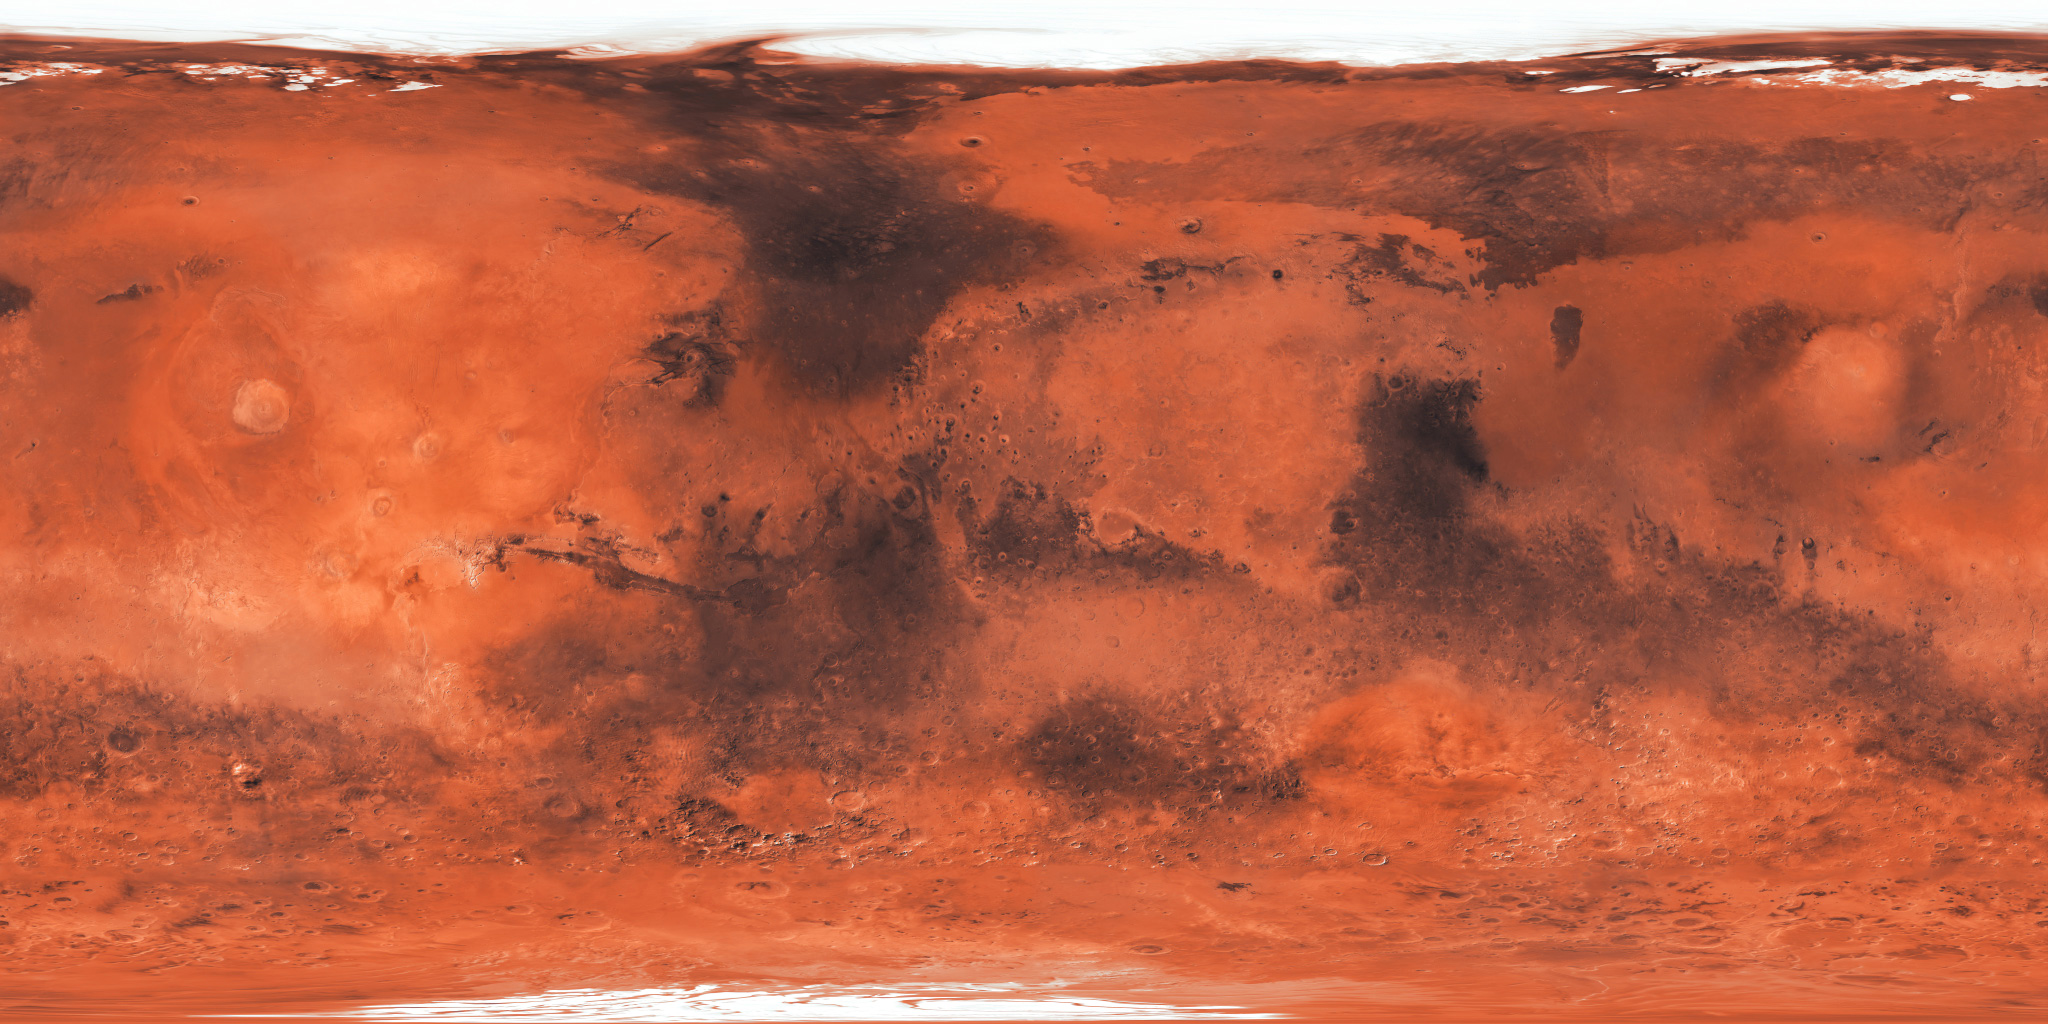
\includegraphics[width=\textwidth]{images/2k_mars.jpg}
            \caption{Tekstura marsa[1]}
            \label{fig:mars}
        \end{figure}
        \FloatBarrier
        \begin{figure}[ht]
            \centering
            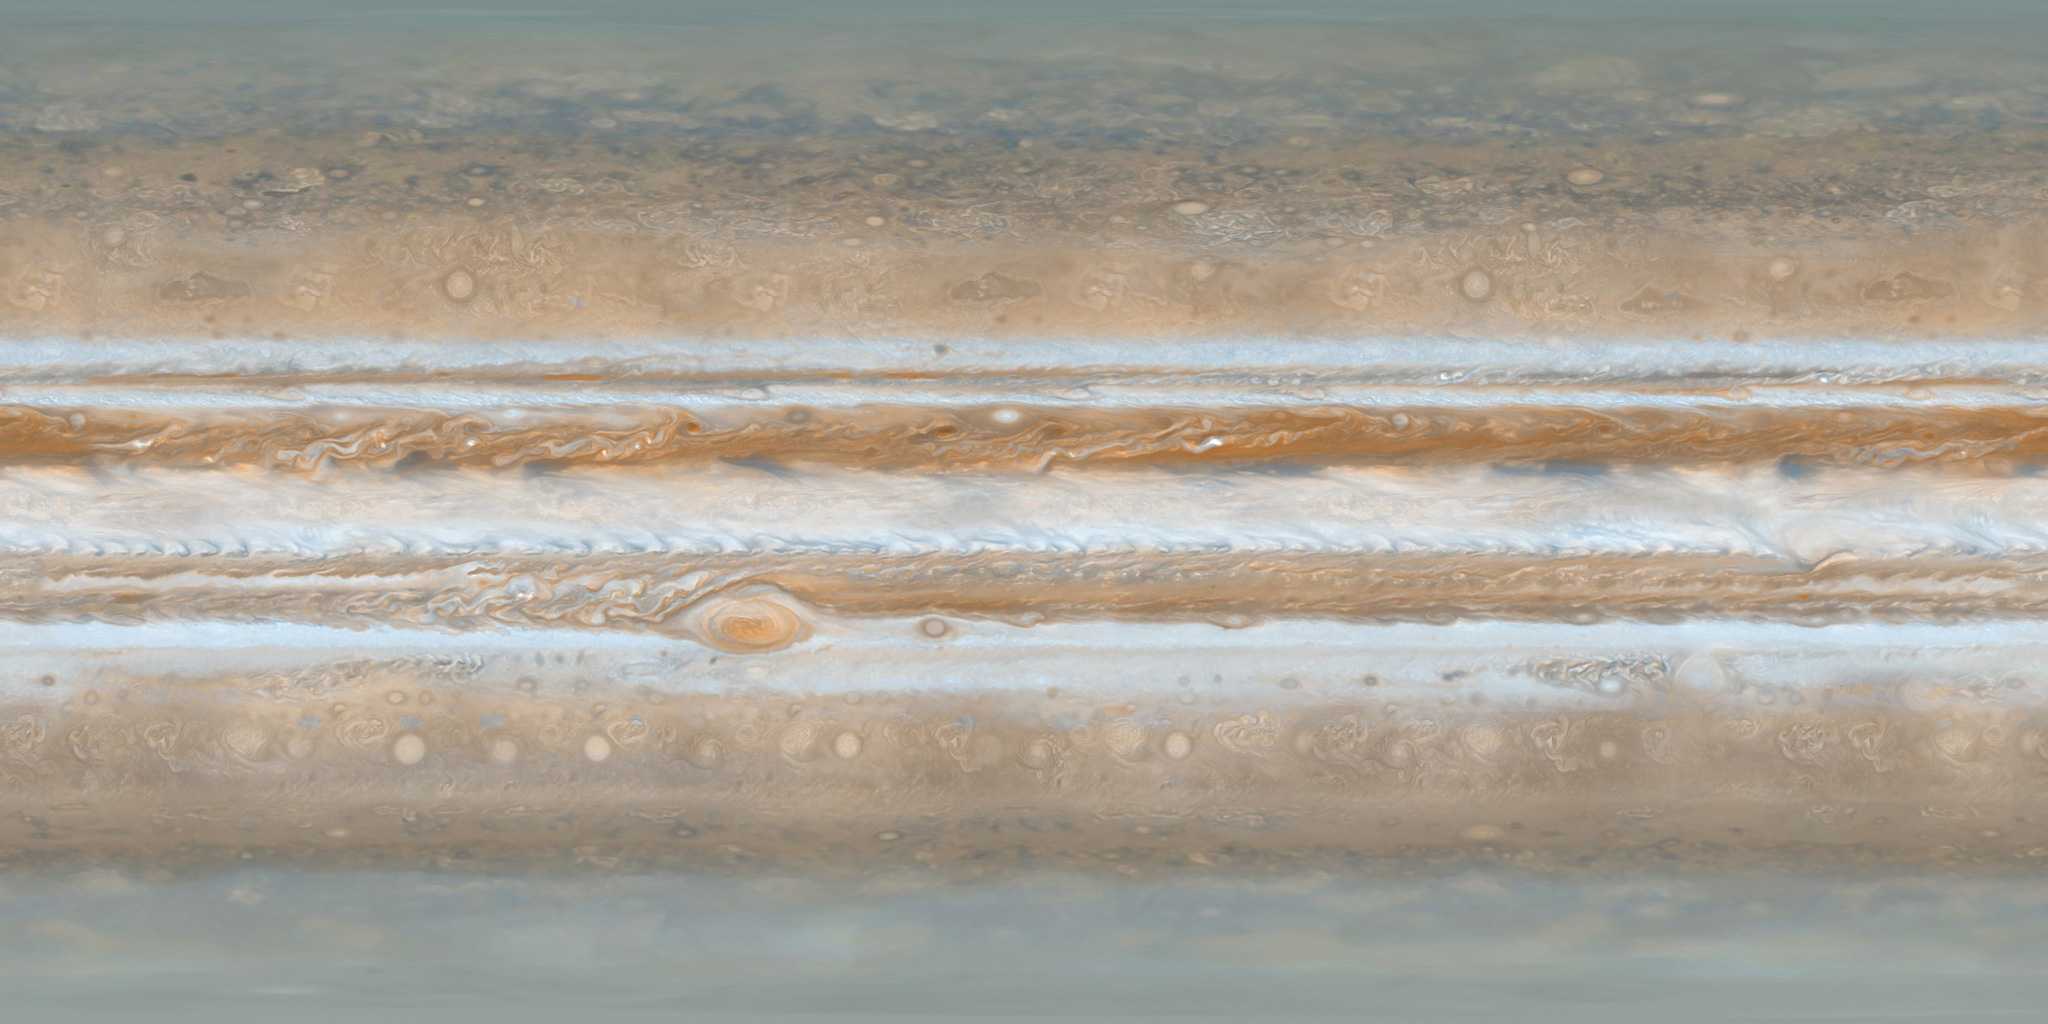
\includegraphics[width=\textwidth]{images/2k_jupiter.jpg}
            \caption{Tekstura jowisza[1]}
            \label{fig:jupiter}
        \end{figure}
        \FloatBarrier
        \begin{figure}[ht]
            \centering
            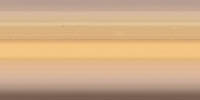
\includegraphics[width=\textwidth]{images/saturnmapthumb.jpg}
            \caption{Tekstura saturna[2]}
            \label{fig:saturn}
        \end{figure}
        \FloatBarrier
        \begin{figure}[ht]
            \centering
            
\includegraphics[width=\textwidth]{images/2k_uranus.jpg}
            \caption{Tekstura urana[1]}
            \label{fig:uranus}
        \end{figure}
        \FloatBarrier
        \begin{figure}[ht]
            \centering
            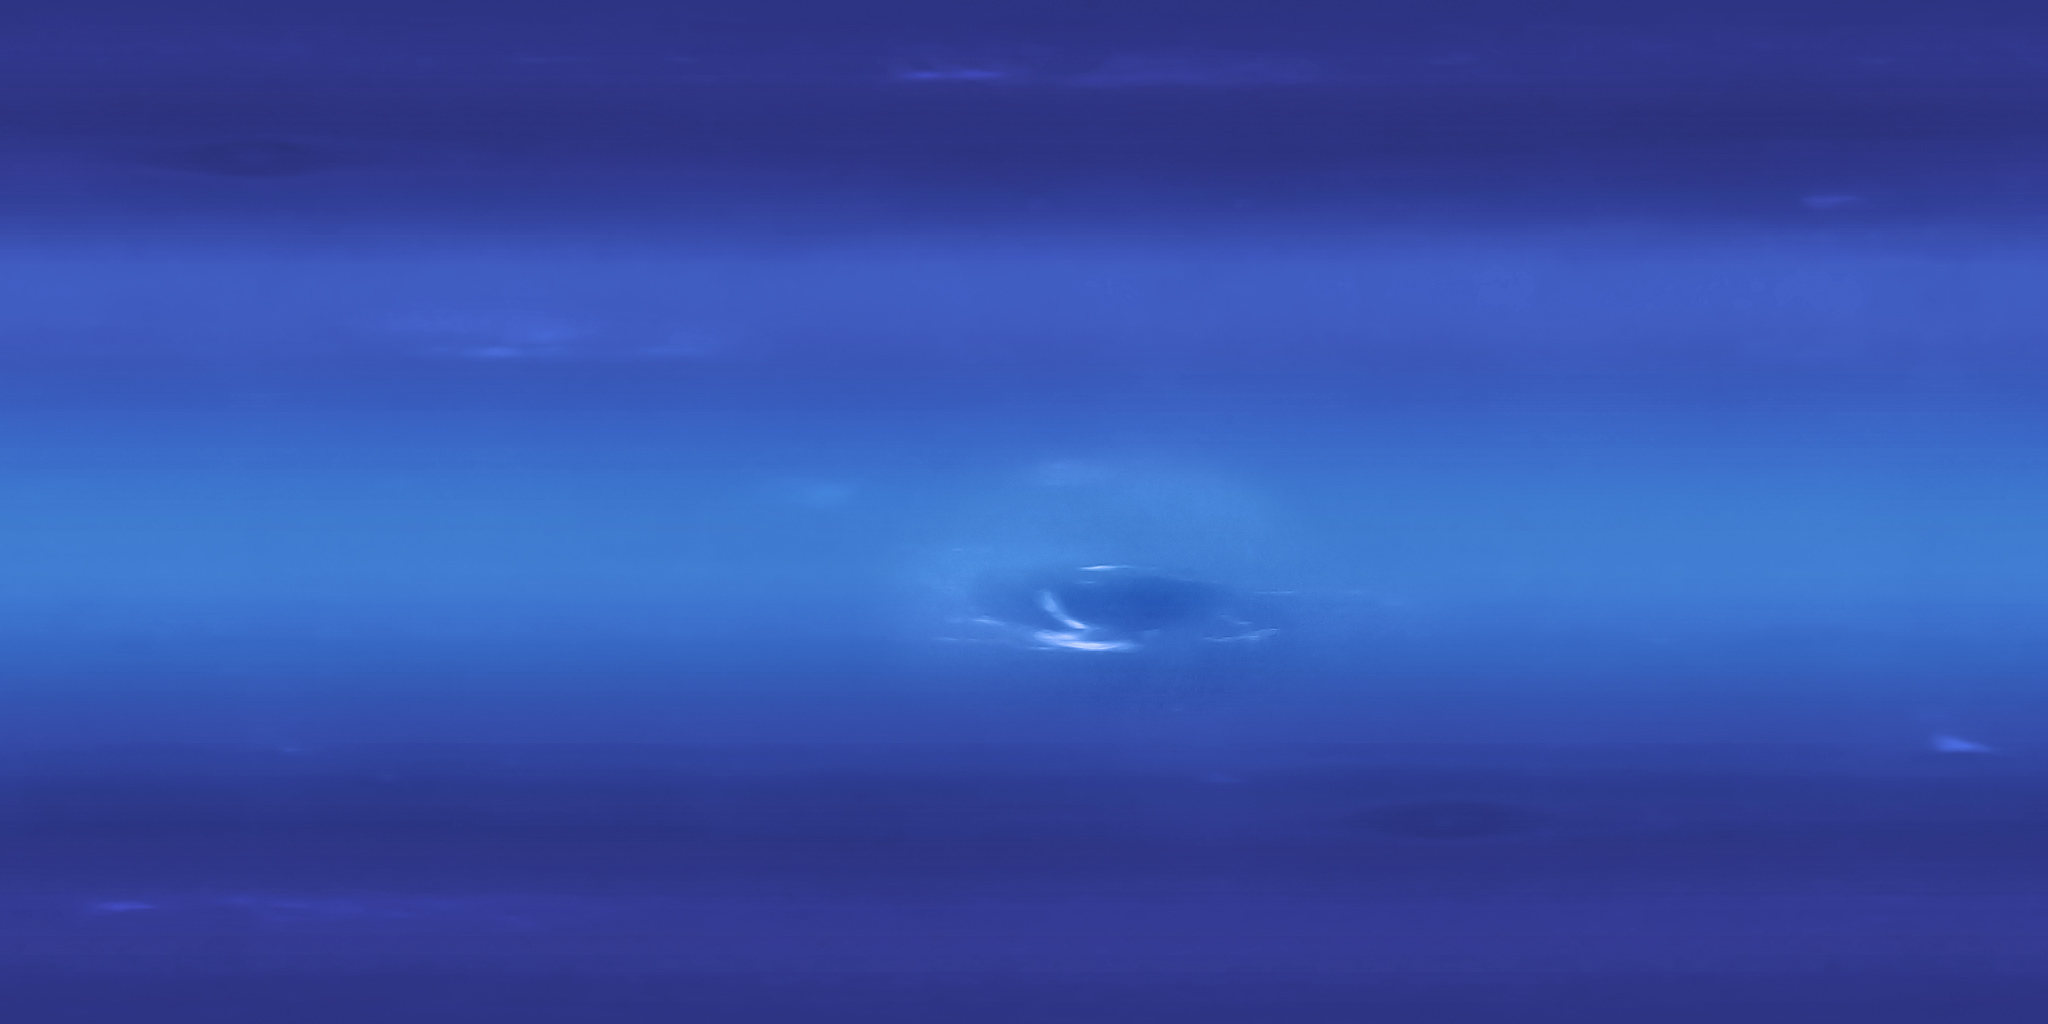
\includegraphics[width=\textwidth]{images/2k_neptune.jpg}
            \caption{Tekstura neptuna[1]}
            \label{fig:neptune}
        \end{figure}
        \FloatBarrier
        \begin{figure}[ht]
            \centering
            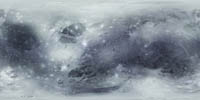
\includegraphics[width=\textwidth]{images/plutomapthumb.jpg}
            \caption{Tekstura pluta[2]}
            \label{fig:pluto}
        \end{figure}
        \FloatBarrier
    \section{Zadanie laboratoryjne}
        \raggedright
        \subsection{Treść zadania}
            W ramach zadania laboratoryjnego należało napisać program symulujący układ słoneczny.
            Symulacja miała składać się z planet wirujących wokół własnej osi Y i jednocześnie 
            orbitujących wokół słońca. Orbita powinna być eliptyczna ze słońcem w jednym z ognisk.
            Ruch po orbicie powinien uwzględniać 3 prawo Keplera. Słońce powinno być źródłem światła.
        \subsection{Opis działania programu}
            Zgodnie z treścią zadania program rysuje 12 obiektów (10 planet,słońce i Księżyc).Wszystkie
            planety obracają się wokół własnej osi i orbitują wokół słońca.
            \textbf{F1} - Zmiana kamery\linebreak
            \textbf{F2} - Poprzednia planeta\linebreak
            \textbf{F3} - Następna planeta\linebreak
            \textbf{F4} - Wypisanie listy planet\linebreak
            \textbf{ESC} - Wyjście z programu\linebreak 
            \textbf{Ruch myszy w osi X} - Obrót kamery w osi X\linebreak 
            \textbf{Ruch myszy w osi Y} - Obrót kamery w osi Y\linebreak 
            \textbf{Scroll up} - Przybiliżenie obiektu\linebreak 
            \textbf{Scroll down} - Oddalenie obiektu\linebreak 
        \subsection{Kod programu}
            \begin{frame}
                \scriptsize
                \inputminted[
                    style={vs},
                    breaklines,
                    breakanywhere, 
                    linenos, 
                    tabsize=4 
                ]{c++}{Lab6.cpp}
                \vspace{1em}
                \captionof{listing}{Fragment kodu z programu}
                \label{lst:Maincode}
            \end{frame}
            \begin{frame}
                \scriptsize
                \inputminted[
                    style={vs},
                    breaklines,
                    breakanywhere, 
                    linenos, 
                    tabsize=4 
                ]{c++}{Planet.cpp}
                \vspace{1em}
                \captionof{listing}{Fragment kodu z programu}
                \label{lst:Planetcode}
            \end{frame}
            \begin{frame}
                \scriptsize
                \inputminted[
                    style={vs},
                    breaklines,
                    breakanywhere, 
                    linenos, 
                    tabsize=4 
                ]{c++}{Sun.cpp}
                \vspace{1em}
                \captionof{listing}{Fragment kodu z programu}
                \label{lst:Suncode}
            \end{frame}
    \section{Wnioski}
    \section{Źródła}
        \begin{enumerate}[label=\arabic*.]
            \item \url{https://www.solarsystemscope.com/textures/}
            \item \url{https://planetpixelemporium.com/pluto.html}
        \end{enumerate}
\end{document}